% !TeX root = ../thesis.tex

\section{Results}

\subsection{RQ1: Probability of failure}\label{ssec:results-rq1}
\autoref{fig:rq1-failure-probability} contains two pie charts that illustrate the amount of failed and successful test runs. The left chart contains the results of the dataset provided by Durieux et al \cite{travisanalysis}. This dataset contains $\SI{4558279}{}$ failed test runs versus $\SI{24323724}{}$ successful runs, which corresponds to a failure probability of $\SI{18.74}{\percent}$. The other pie chart visualises data from the TravisTorrent project. According to this dataset, the run has failed prior to starting the test suite in $\SI{42.89}{\percent}$ of the executions. For the remaining part of the runs, $\SI{225766}{}$ out of $\SI{2114920}{}$ executions contained at least one failed test case, corresponding to a failure percentage of $\SI{10.67}{\percent}$.

\begin{figure}[htbp!]
	\centering
	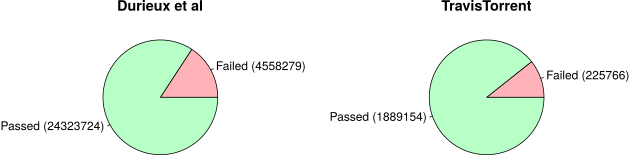
\includegraphics[width=\textwidth]{assets/charts/rq1-failure-probability.pdf}
	\caption{Probability of test run failure}
	\label{fig:rq1-failure-probability}
\end{figure}

\subsection{RQ2: Probability of consecutive failure}
In order to find consecutive failures, only the TravisTorrent project can be used as every entry in this dataset contains the identifier of the previous build which is required to link consecutive builds. The dataset contains $\SI{211040}{}$ test runs of which the test suite of the preceding test run was both executed and contained at least one failed test case. As illustrated in \autoref{fig:rq2-consecutive-failure}, $\SI{109224}{}$ of these test runs failed as well, versus $\SI{101816}{}$ test runs ($\SI{51.76}{\percent}$) that did succeed.

\begin{figure}[htbp!]
	\centering
	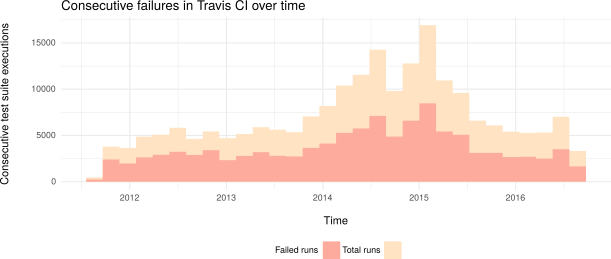
\includegraphics[width=\textwidth]{assets/charts/rq2-consecutive-failure.pdf}
	\caption{Consecutive test run failures on \travisci{}}
	\label{fig:rq2-consecutive-failure}
\end{figure}

\subsection{RQ3: Average test run duration}
The \travisci{} dataset provided by Durieux et al \cite{travisanalysis} has been filtered to exclude test runs with an execution time of less than $\SI{10}{\second}$, as this generally implies that the test suite did not actually execute due to an initialisation failure. \autoref{tbl:rq3-characteristics} contains the characteristics of the remaining analysed test runs. This table suggests that \travisci{} is primarily used for small projects, yet the maximal value is a strong outlier. \autoref{fig:rq3-durations} confirms the existence of $\SI{71378}{}$ test runs with an execution time of more than one hour. Further investigation has pointed out that these are mostly projects which are using mutation testing (\autoref{sssec:mutation-testing}), such as \texttt{plexus/yaks}\footnote{A Ruby library for hypermedia (\url{https://github.com/plexus/yaks}).}.

\begin{table}[h]
	\centering
	\begin{tabularx}{\textwidth}{|C|C|C|C|C|}
		\hline
		\textbf{\# runs} & \textbf{Minimum} & \textbf{Mean} & \textbf{Median} & \textbf{Maximum}\\
		\hline
		$\SI{24320504}{}$ & $\SI{10}{\second}$ & $\SI{385}{\second}$ & $\SI{178}{\second}$ & $\SI{26}{\hour} \SI{11}{\minute} \SI{26}{\second}$\\
		\hline
	\end{tabularx}
	\caption{Characteristics of the test run durations in \cite{travisanalysis}.}
	\label{tbl:rq3-characteristics}
\end{table}

\begin{figure}[htbp!]
	\centering
	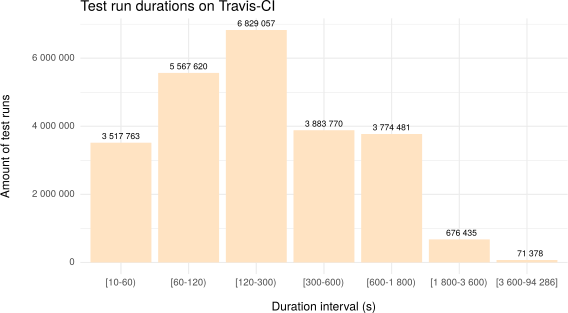
\includegraphics[width=\textwidth]{assets/charts/rq3-test-run-durations.pdf}
	\caption{Test run durations on \travisci{}}
	\label{fig:rq3-durations}
\end{figure}


\subsection{RQ4: Applying \tcp{} to Dodona}
Given the $\SI{62}{}$ collected test runs, another $\SI{9}{}$ runs have been omitted because these have been identified as a bug in the configuration of the test suite, preventing any test to be executed at all. This is something which cannot be detected by a prioritisation framework, since this requires more contextual information about the project.\\

\noindent \autoref{fig:rq4-performance} compares the performance of respectively the Alpha algorithm, the Greedy algorithm, the HGS algorithm and the ROCKET algorithm to the original, non-prioritised execution. The Alpha and HGS algorithm provide the most accurate predictions, with the latter algorithm being the least consistent. The Greedy algorithm on the other hand succeeds in predicting some executions very accurately, while failing to predict other runs anywhere near, which is the expected behaviour of a greedy heuristic. Finally, the ROCKET algorithm is not suitable for this project.\\

\begin{figure}[htbp!]
\centering
\subfloat[Alpha algorithm]{%
	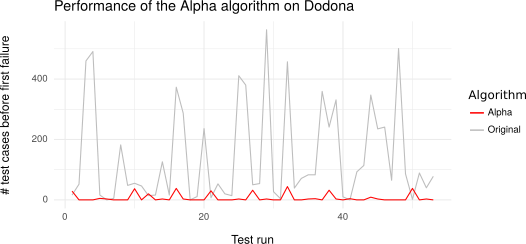
\includegraphics[width=\textwidth]{assets/charts/rq4-dodona-alpha.pdf}
}
\end{figure}
\begin{figure}
\ContinuedFloat
\subfloat[Greedy algorithm]{%
	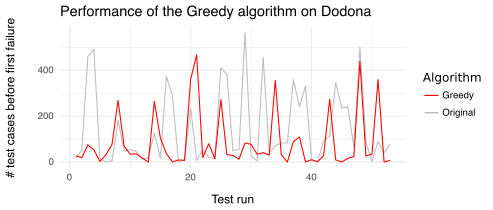
\includegraphics[width=\textwidth]{assets/charts/rq4-dodona-greedy.pdf}
}
\end{figure}
\begin{figure}
\ContinuedFloat
\subfloat[HGS algorithm]{%
	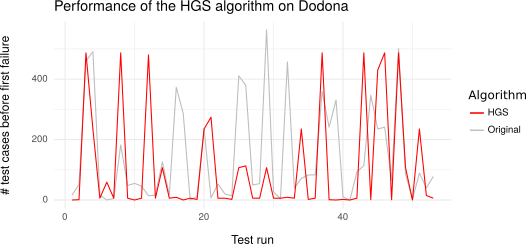
\includegraphics[width=\textwidth]{assets/charts/rq4-dodona-hgs.pdf}
}
\end{figure}
\begin{figure}
\ContinuedFloat
\centering
\subfloat[ROCKET algorithm]{%
	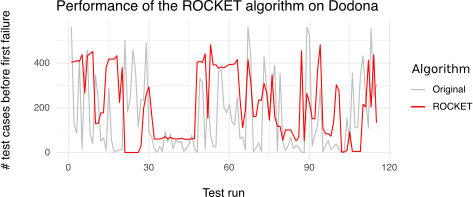
\includegraphics[width=\textwidth]{assets/charts/rq4-dodona-rocket.pdf}
}
\caption{Prediction performance on the Dodona project}
\label{fig:rq4-performance}
\end{figure}

\noindent \autoref{tbl:rq4-first-failure} contains the minimum, mean, median and maximum median amount of test cases until the first failure is observed. This table indicates that, except for the GreedyCoverAffected algorithm\footnote{The AllInOrder algorithm can be considered a deterministic random algorithm and therefore not an actual predictor.}, every predictor is able to perform at least one successful prediction. Furthermore, the maximum amount of executed test cases is lower than the original, for every predictor. The previous paragraph has already observed that the Alpha and HGS algorithm provide the best prediction accuracy for Dodona, this hypothesis is confirmed by the low median and mean values for these algorithms. These values confirm as well that the ROCKET algorithm is not able of providing accurate predictions.

\begin{table}[h]
	\centering
	\begin{tabularx}{\textwidth}{|X||c|c|c|c|}
		\hline
		\textbf{Algorithm} & \textbf{Minimum} & \textbf{Mean} & \textbf{Median} & \textbf{Maximum}\\
		
		\hline
		
		\emph{Original} & $\SI{0}{}$ & $\SI{143}{}$ & $\SI{65}{}$ & $\SI{563}{}$\\
		
		\hline
		
		Alpha & $\SI{0}{}$ & $\SI{7}{}$ & $\SI{6}{}$ & $\SI{44}{}$\\
		
		\hline
		AffectedRandom & $\SI{0}{}$ & $\SI{82}{}$ & $\SI{18}{}$ & $\SI{428}{}$\\
		AllInOrder & $\SI{1}{}$ & $\SI{102}{}$ & $\SI{71}{}$ & $\SI{455}{}$\\
		AllRandom & $\SI{0}{}$ & $\SI{71}{}$ & $\SI{16}{}$ & $\SI{477}{}$\\
		
		\hline
		
		GreedyCoverAffected & $\SI{31}{}$ & $\SI{307}{}$ & $\SI{296}{}$ & $\SI{446}{}$\\
		GreedyCoverAll & $\SI{0}{}$ & $\SI{85}{}$ & $\SI{32}{}$ & $\SI{467}{}$\\
		GreedyTimeAll & $\SI{0}{}$ & $\SI{209}{}$ & $\SI{172}{}$ & $\SI{452}{}$\\
		
		\hline
		
		HGSAffected & $\SI{0}{}$ & $\SI{54}{}$ & $\SI{10}{}$ & $\SI{511}{}$\\
		HGSAll & $\SI{0}{}$ & $\SI{109}{}$ & $\SI{6}{}$ & $\SI{487}{}$\\
		
		\hline
		
		ROCKET & $\SI{0}{}$ & $\SI{208}{}$ & $\SI{170}{}$ & $\SI{452}{}$\\
		
		\hline
	\end{tabularx}
	\caption{Amount of executed test cases until the first failure.}
	\label{tbl:rq4-first-failure}
\end{table}

\noindent Similarly, \autoref{tbl:rq4-first-failure-duration} contains the minimum, mean, maximum and median duration until the first failed test case is observed. This data further confirms the observations made in the previous paragraph and the effectiveness of the GreedyTimeAll predictor. Notice that the ROCKET algorithm performs better time-wise than quantity wise.

\begin{table}[h]
	\centering
	\begin{tabularx}{\textwidth}{|X||c|c|c|c|}
		\hline
		\textbf{Algorithm} & \textbf{Minimum} & \textbf{Mean} & \textbf{Median} & \textbf{Maximum}\\
		
		\hline
		
		\emph{Original} & $\SI{0}{\second}$ & $\SI{154}{\second}$ & $\SI{125}{\second}$ & $\SI{622}{\second}$\\
		
		\hline
		
		Alpha & $\SI{0}{\second}$ & $\SI{5}{\second}$ & $\SI{0}{\second}$ & $\SI{84}{\second}$\\
		
		\hline
		AffectedRandom & $\SI{0}{\second}$ & $\SI{64}{\second}$ & $\SI{10}{\second}$ & $\SI{355}{\second}$\\
		AllInOrder & $\SI{0}{\second}$ & $\SI{177}{\second}$ & $\SI{171}{\second}$ & $\SI{456}{\second}$\\
		AllRandom & $\SI{0}{\second}$ & $\SI{64}{\second}$ & $\SI{11}{\second}$ & $\SI{611}{\second}$\\
		
		\hline
		
		GreedyCoverAffected & $\SI{6}{\second}$ & $\SI{123}{\second}$ & $\SI{109}{\second}$ & $\SI{264}{\second}$\\
		GreedyCoverAll & $\SI{0}{\second}$ & $\SI{60}{\second}$ & $\SI{25}{\second}$ & $\SI{306}{\second}$\\
		GreedyTimeAll & $\SI{0}{\second}$ & $\SI{44}{\second}$ & $\SI{15}{\second}$ & $\SI{178}{\second}$\\
		
		\hline
		
		HGSAffected & $\SI{0}{\second}$ & $\SI{58}{\second}$ & $\SI{6}{\second}$ & $\SI{581}{\second}$\\
		HGSAll & $\SI{0}{\second}$ & $\SI{130}{\second}$ & $\SI{16}{\second}$ & $\SI{578}{\second}$\\
		
		\hline
		
		ROCKET & $\SI{0}{\second}$ & $\SI{47}{\second}$ & $\SI{16}{\second}$ & $\SI{178}{\second}$\\
		
		\hline
	\end{tabularx}
	\caption{Duration until the first failure.}
	\label{tbl:rq4-first-failure-duration}
\end{table}

    duration         Original        AllRandom     
Min.   :118165   Min.   :  0.00   Min.   : 0.000  
1st Qu.:195877   1st Qu.:  0.00   1st Qu.: 0.000  
Median :297371   Median :  2.00   Median : 4.000  
Mean   :303527   Mean   : 67.57   Mean   : 9.257  
3rd Qu.:414956   3rd Qu.:110.00   3rd Qu.:13.500  
Max.   :505996   Max.   :278.00   Max.   :64.000  

AllInOrder     GreedyCoverAll   AffectedRandom  
Min.   : 0.000   Min.   : 0.000   Min.   : 0.000  
1st Qu.: 0.000   1st Qu.: 0.000   1st Qu.: 0.000  
Median : 1.000   Median : 1.000   Median : 2.000  
Mean   : 9.229   Mean   : 8.971   Mean   : 8.886  
3rd Qu.:12.000   3rd Qu.:13.000   3rd Qu.:11.500  
Max.   :37.000   Max.   :44.000   Max.   :45.000  

HGSAffected     GreedyCoverAffected     HGSAll    
Min.   : 0.000   Min.   : 0.00       Min.   : 0.0  
1st Qu.: 0.000   1st Qu.: 0.00       1st Qu.: 0.0  
Median : 3.000   Median : 2.00       Median : 7.0  
Mean   : 8.886   Mean   :15.09       Mean   : 9.6  
3rd Qu.:11.500   3rd Qu.:31.00       3rd Qu.:12.5  
Max.   :64.000   Max.   :43.00       Max.   :43.0  

Alpha            Rocket       GreedyTimeAll   
Min.   : 0.000   Min.   :  0.00   Min.   :  0.00  
1st Qu.: 0.000   1st Qu.:  3.50   1st Qu.:  3.50  
Median : 1.000   Median : 27.00   Median : 27.00  
Mean   : 8.971   Mean   : 42.23   Mean   : 42.23  
3rd Qu.:13.000   3rd Qu.: 49.00   3rd Qu.: 49.00  
Max.   :44.000   Max.   :216.00   Max.   :216.00  

Original\_ms      AllRandom\_ms    AllInOrder\_ms   
Min.   :     0   Min.   :     0   Min.   :     0  
1st Qu.:     0   1st Qu.:     0   1st Qu.:     0  
Median :  9560   Median :   739   Median :   862  
Mean   : 73612   Mean   : 13299   Mean   : 32391  
3rd Qu.:122586   3rd Qu.: 13592   3rd Qu.: 78063  
Max.   :283433   Max.   :184805   Max.   :139345  

GreedyCoverAll\_ms AffectedRandom\_ms HGSAffected\_ms  
Min.   :     0    Min.   :     0    Min.   :     0  
1st Qu.:     0    1st Qu.:     0    1st Qu.:     0  
Median :   620    Median :   317    Median :  1318  
Mean   : 15251    Mean   : 19732    Mean   : 23738  
3rd Qu.:  8620    3rd Qu.:  6460    3rd Qu.: 11786  
Max.   :197463    Max.   :174491    Max.   :211702  

GreedyCoverAffected\_ms   HGSAll\_ms         Alpha\_ms     
Min.   :    0          Min.   :     0   Min.   :     0  
1st Qu.:    0          1st Qu.:     0   1st Qu.:     0  
Median : 4229          Median :  2818   Median :   647  
Mean   :21835          Mean   : 12494   Mean   : 15189  
3rd Qu.:37885          3rd Qu.:  8475   3rd Qu.:  8386  
Max.   :75637          Max.   :157003   Max.   :193618  

Rocket\_ms      GreedyTimeAll\_ms      idx      
Min.   :     0   Min.   :    0    Min.   : 1.0  
1st Qu.:     0   1st Qu.:    0    1st Qu.: 9.5  
Median :   254   Median :  257    Median :18.0  
Mean   :  6844   Mean   : 6852    Mean   :18.0  
3rd Qu.:  1760   3rd Qu.: 1754    3rd Qu.:26.5  
Max.   :100011   Max.   :99765    Max.   :35.0  
